\documentclass{beamer}\usepackage[]{graphicx}\usepackage[]{color}
% maxwidth is the original width if it is less than linewidth
% otherwise use linewidth (to make sure the graphics do not exceed the margin)
\makeatletter
\def\maxwidth{ %
  \ifdim\Gin@nat@width>\linewidth
    \linewidth
  \else
    \Gin@nat@width
  \fi
}
\makeatother

\definecolor{fgcolor}{rgb}{0.345, 0.345, 0.345}
\newcommand{\hlnum}[1]{\textcolor[rgb]{0.686,0.059,0.569}{#1}}%
\newcommand{\hlstr}[1]{\textcolor[rgb]{0.192,0.494,0.8}{#1}}%
\newcommand{\hlcom}[1]{\textcolor[rgb]{0.678,0.584,0.686}{\textit{#1}}}%
\newcommand{\hlopt}[1]{\textcolor[rgb]{0,0,0}{#1}}%
\newcommand{\hlstd}[1]{\textcolor[rgb]{0.345,0.345,0.345}{#1}}%
\newcommand{\hlkwa}[1]{\textcolor[rgb]{0.161,0.373,0.58}{\textbf{#1}}}%
\newcommand{\hlkwb}[1]{\textcolor[rgb]{0.69,0.353,0.396}{#1}}%
\newcommand{\hlkwc}[1]{\textcolor[rgb]{0.333,0.667,0.333}{#1}}%
\newcommand{\hlkwd}[1]{\textcolor[rgb]{0.737,0.353,0.396}{\textbf{#1}}}%
\let\hlipl\hlkwb

\usepackage{framed}
\makeatletter
\newenvironment{kframe}{%
 \def\at@end@of@kframe{}%
 \ifinner\ifhmode%
  \def\at@end@of@kframe{\end{minipage}}%
  \begin{minipage}{\columnwidth}%
 \fi\fi%
 \def\FrameCommand##1{\hskip\@totalleftmargin \hskip-\fboxsep
 \colorbox{shadecolor}{##1}\hskip-\fboxsep
     % There is no \\@totalrightmargin, so:
     \hskip-\linewidth \hskip-\@totalleftmargin \hskip\columnwidth}%
 \MakeFramed {\advance\hsize-\width
   \@totalleftmargin\z@ \linewidth\hsize
   \@setminipage}}%
 {\par\unskip\endMakeFramed%
 \at@end@of@kframe}
\makeatother

\definecolor{shadecolor}{rgb}{.97, .97, .97}
\definecolor{messagecolor}{rgb}{0, 0, 0}
\definecolor{warningcolor}{rgb}{1, 0, 1}
\definecolor{errorcolor}{rgb}{1, 0, 0}
\newenvironment{knitrout}{}{} % an empty environment to be redefined in TeX

\usepackage{alltt}
\usetheme{Boadilla}

\makeatother
\setbeamertemplate{footline}
{
    \leavevmode%
    \hbox{%
    \begin{beamercolorbox}[wd=.4\paperwidth,ht=2.25ex,dp=1ex,center]{author in head/foot}%
        \usebeamerfont{author in head/foot}\insertshortauthor
    \end{beamercolorbox}%
    \begin{beamercolorbox}[wd=.55\paperwidth,ht=2.25ex,dp=1ex,center]{title in head/foot}%
        \usebeamerfont{title in head/foot}\insertshorttitle
    \end{beamercolorbox}%
    \begin{beamercolorbox}[wd=.05\paperwidth,ht=2.25ex,dp=1ex,center]{date in head/foot}%
        \insertframenumber{}
    \end{beamercolorbox}}%
    \vskip0pt%
}
\makeatletter
\setbeamertemplate{navigation symbols}{}

\usepackage{lmodern}
\usepackage{amssymb,amsmath}
\renewcommand{\familydefault}{\sfdefault}

\usepackage{mathtools}
\usepackage{graphicx}
\usepackage{threeparttable}
\usepackage{booktabs}
\usepackage{siunitx}
\sisetup{parse-numbers=false}

\setlength{\OuterFrameSep}{-2pt}
\makeatletter
\preto{\@verbatim}{\topsep=-10pt \partopsep=-10pt }
\makeatother

\title[Lecture 1:\ Introduction]{Lecture 1:\ Introduction}
\author[ResEcon 703:\ Advanced Econometrics]{ResEcon 703:\ Topics in Advanced Econometrics}
\date{Matt Woerman\\University of Massachusetts Amherst}
\IfFileExists{upquote.sty}{\usepackage{upquote}}{}
\begin{document}


{\setbeamertemplate{footline}{} 
\begin{frame}[noframenumbering]
    \titlepage
\end{frame}
}

\begin{frame}\frametitle{Agenda}
    Today
    \begin{itemize}
        \item Course overview
        \item What is ``structural estimation?''
        \item Getting started with R
    \end{itemize}
    \vspace{3ex}
    Upcoming
    \begin{itemize}
        \item For next time
        \begin{itemize}
            \item Reiss and Wolack (2007), Sections 1--4
            \item Install R software
        \end{itemize}
    \end{itemize}
\end{frame}

\begin{frame}\frametitle{}
    \vfill
    \centering
    \begin{beamercolorbox}[center]{title}
        \Large Course Overview
    \end{beamercolorbox}
    \vfill
\end{frame}

\begin{frame}\frametitle{Course Website}
    \begin{center}
        \href{https://github.com/woerman/ResEcon703}{\texttt{github.com/woerman/ResEcon703}}
    \end{center}
    \vspace{3ex}
    I will use this GitHub repository to post lecture slides, R code, problem sets, datasets, etc.
\end{frame}

\begin{frame}\frametitle{My Info}
    Matt Woerman
    \begin{itemize}
        \item Email: \href{mailton:mwoerman@umass.edu}{\texttt{mwoerman@umass.edu}}
        \item Office: 218 Stockbridge Hall
        \item Office hours: Tuesday, 2:00--3:00 pm
    \end{itemize}
    \vspace{3ex}
    Best way to communicate with me
    \begin{itemize}
        \item Short public question: Ask in class
        \item Short private question: Email with [ResEcon 703] in the subject
        \item Longer question: Come to office hours
    \end{itemize}
\end{frame}

\begin{frame}\frametitle{About Me}
    \begin{itemize}
        \item I study energy and environmental economics, industrial organization, and applied econometrics
        \begin{itemize}
            \item Market power in wholesale electricity markets
            \item Role of electricity in agricultural groundwater extraction
            \item Design of carbon markets and other environmental policies
            \item Tools for designing field experiments using panel data
        \end{itemize}
        \item This is my first year as a professor and first time teaching this course
        \begin{itemize}
            \item You can play a role in shaping the design of this course, for yourself and for future classes!
        \end{itemize}
        \item My wife is a professor in the Biology Department at UMass
        \begin{itemize}
            \item ``Dr.\ Woerman'' is not a unique identifier, so call me ``Matt''
        \end{itemize}
        \item Pronouns: he/him/his
    \end{itemize}
\end{frame}

\begin{frame}\frametitle{About You}
    Introduce yourself
    \begin{itemize}
        \item Name
        \item Pronouns
        \item Department
        \item Research interests
        \item Anything else you want us to know?
    \end{itemize}
\end{frame}

\begin{frame}\frametitle{Course Description}
    You've already taken
    \begin{itemize}
        \item ResEcon 701: Probability Theory and Statistical Inference
        \item ResEcon 702: Econometric Methods
        \begin{itemize}
            \item Classical linear regression model
            \item ``Treatment effect'' estimation
        \end{itemize}
    \end{itemize}
    (If you have not taken ResEcon 702, please see me to determine if this course is appropriate for you) \\
    \vspace{3ex}
    Isn't that enough? What else is there?
    \begin{itemize}
        \item Nonlinear regression models 
        \item Structural estimation
        \item Discrete choice models
    \end{itemize}
\end{frame}

\begin{frame}\frametitle{Course Goals}
    \begin{enumerate}
        \item Gain an in-depth understanding of the most common structural estimation methods in modern empirical economics
        \begin{itemize}
            \item Maximum likelihood estimation
            \item Nonlinear least squares
            \item Generalized method of moments
        \end{itemize}
        \vspace{1ex} 
        \item Develop the technical ability to apply these methods to your own research
        \vspace{1ex}
        \item Apply these methods to discrete choice models motivated by the random utility model
        \begin{itemize}
            \item Logit model
            \item Generalized extreme value models (nested logit)
            \item Mixed logit model (random coefficients logit model)
        \end{itemize}
    \end{enumerate}
\end{frame}

\begin{frame}\frametitle{Textbooks}
    \begin{tabular}{cl}  
        \begin{tabular}{c}
            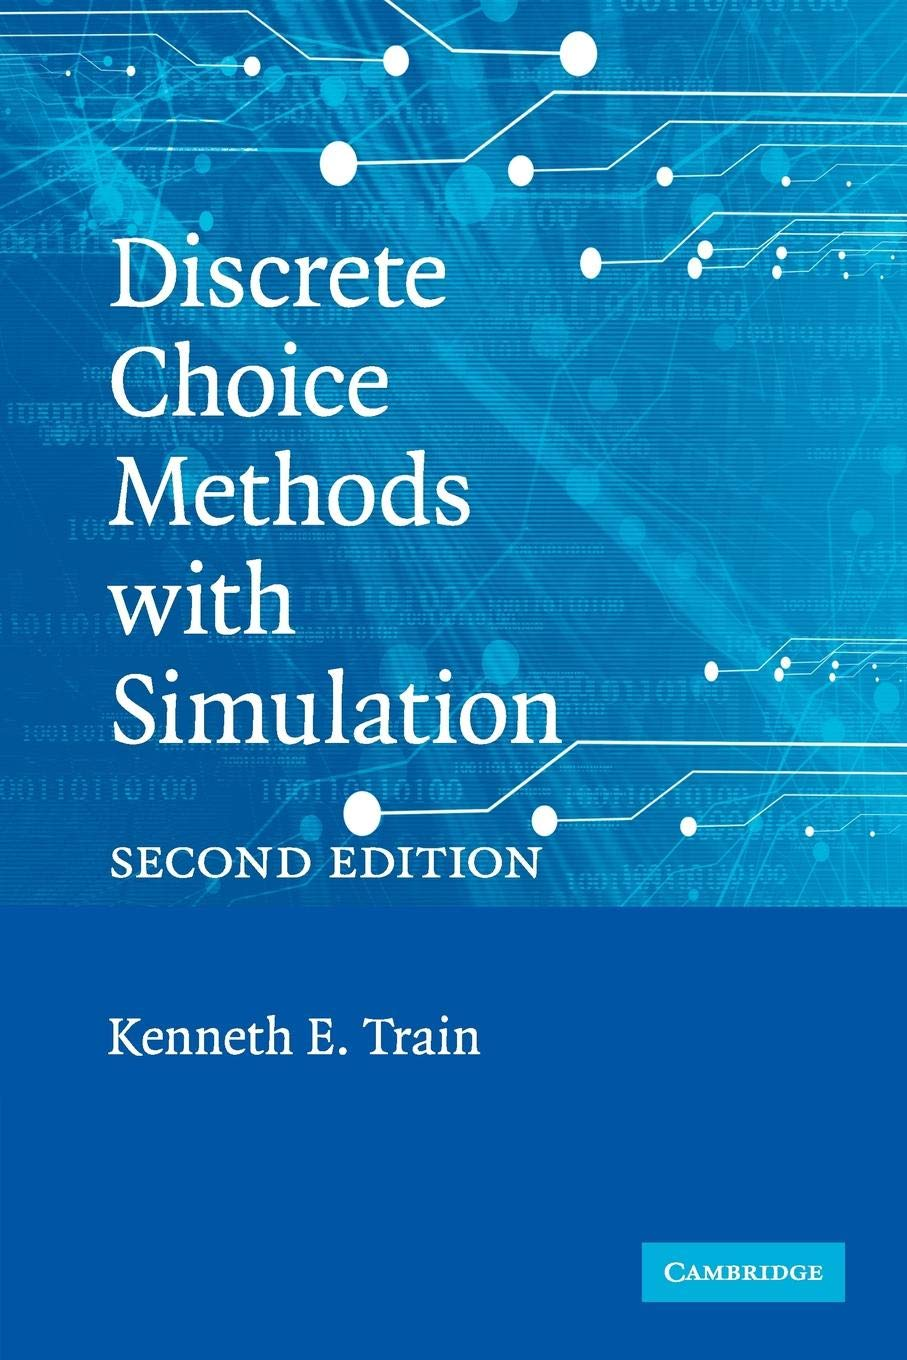
\includegraphics[width=0.2\linewidth]{train}
        \end{tabular} & 
        \begin{tabular}{l}
            \parbox{0.65\linewidth}{
            \emph{Discrete Choice Methods with Simulation\\ (Second Edition)} by Kenneth E.\ Train
            \begin{itemize}
                \item Available for free at: \href{https://eml.berkeley.edu/books/choice2.html}{\texttt{eml.berkeley.edu/books/choice2.html}}
                \item Paperback copy is only \$40
            \end{itemize}
            }
        \end{tabular}
    \end{tabular} \\
    \vspace{1ex}
    \begin{tabular}{cl}  
        \begin{tabular}{c}
            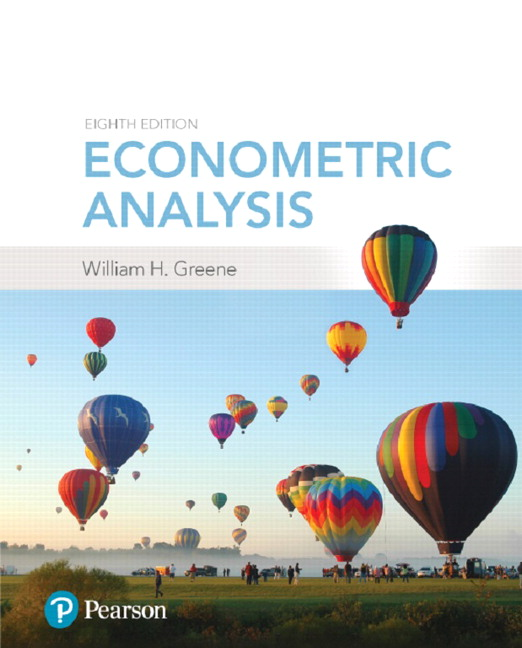
\includegraphics[width=0.2\linewidth]{greene}
        \end{tabular} & 
        \begin{tabular}{l}
            \parbox{0.65\linewidth}{
            \emph{Econometric Analysis (Eighth Edition)}\\ by William H. Greene
            \begin{itemize}
                \item Same textbook you used in ResEcon 702
                \item Seventh Edition is also fine
            \end{itemize}
            }
        \end{tabular}
    \end{tabular}
\end{frame}

\begin{frame}\frametitle{Other References}
    \begin{tabular}{cl}  
        \begin{tabular}{c}
            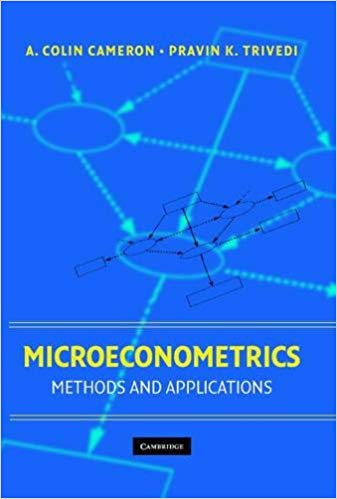
\includegraphics[width=0.2\linewidth]{cameron}
        \end{tabular} & 
        \begin{tabular}{l}
            \parbox{0.65\linewidth}{
            \emph{Microeconometrics:\ Methods and Applications}\\ by A. Colin Cameron and Pravin K. Trivedi
            \begin{itemize}
                \item More applied than many econometrics texts
            \end{itemize}
            }
        \end{tabular}
    \end{tabular} \\
    \vspace{1ex}
    \begin{tabular}{cl}  
        \begin{tabular}{c}
            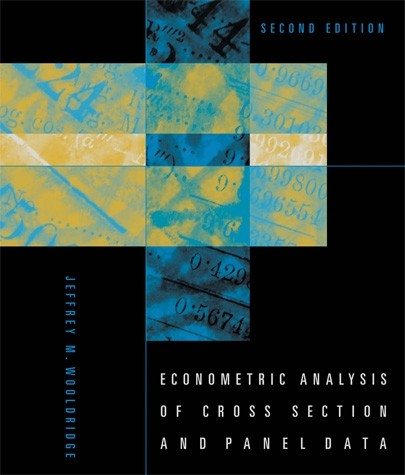
\includegraphics[width=0.2\linewidth]{wooldridge}
        \end{tabular} & 
        \begin{tabular}{l}
            \parbox{0.66\linewidth}{
            \emph{Econometric Analysis of Cross Section and Panel Data (Second Edition)} by Jeffrey M. Wooldridge
            \begin{itemize}
                \item More advanced material than other textbooks
            \end{itemize}
            }
        \end{tabular}
    \end{tabular}
\end{frame}

\begin{frame}\frametitle{Readings}
    We will read papers to see how these structural estimation methods have been applied to
    \begin{itemize}
        \item Energy economics
        \item Environmental economics
        \item Experimental economics
        \item Health economics
        \item Industrial organization
        \item Labor economics
        \item Public economics
    \end{itemize}
\end{frame}

\begin{frame}\frametitle{Software}
    We will use the R statistical programming language in this course \\
    \vspace{1.5ex}
    But I already know Stata/Matlab/Python/SAS/Julia. Why R?
    \begin{itemize}
        \item R is free and open source
        \item R is powerful and flexible
        \begin{itemize}
            \item Basic statistics, data cleaning, linear regression, matrix algebra, simulation methods, structural estimation, data visualization, etc.
        \end{itemize}
        \item R is favored by employers
    \end{itemize}
    \vspace{1.5ex}
    How can I learn R?
    \begin{itemize}
        \item R tutorial next class
        \item Many R resources available for free
        \item First problem set will be a (relatively) gentle introduction to R
    \end{itemize}
    \vspace{1.5ex}
    You do not have to use R. But I will not provide any support or partial credit for work done in other programming languages.
\end{frame}

\begin{frame}\frametitle{Grades}
    Your final grade will be made up of
    \begin{itemize}
        \item Problem sets: 4 at 15\% each (60\% total)
        \item Final exam: 30\%
        \item Attendance and participation: 10\%
    \end{itemize}
\end{frame}

\begin{frame}\frametitle{Problem Sets}
    Problems sets will simulate the kind of analysis you will do when conducting your own research
    \begin{itemize}
        \item Apply the estimation methods you learn in class
        \item Interpret your results
        \item Draw policy-relevant conclusions
    \end{itemize}
    \vspace{3ex}
    Rules for problem sets
    \begin{itemize}
        \item You can work in groups of up to three people (I recommend you do)
        \item Each person must submit a unique set of answers
        \item You must submit your code with your write up
        \item You can only use ``canned'' routines when told to do so
    \end{itemize}
    \vspace{3ex}
    See syllabus for tentative problem set schedule
\end{frame}

\begin{frame}\frametitle{Final Exam}
    Final exam will be similar to problem sets
    \begin{itemize}
        \item Take-home, not in class
        \item Estimation, interpretation, etc.
        \item At least a week to complete (actual exam timeline TBD)
    \end{itemize}
    \vspace{3ex}
    How the final exam differs from problem sets
    \begin{itemize}
        \item Will require roughly twice the effort of a problem set
        \item SINGLE-AUTHORED! No collaboration, consultation, etc.
    \end{itemize}
    \vspace{3ex}
    More details to come toward the end of the semester
\end{frame}

\begin{frame}\frametitle{Attendance and Participation}
    Attendance is required
    \begin{itemize}
        \item You can miss at most two lectures and still receive full points
    \end{itemize}
    \vspace{3ex}
    ``Participation'' is required
    \begin{itemize}
        \item Come to class prepared
        \item Complete the reading before class
        \item Bring your laptop to work through examples together
    \end{itemize}
    \vspace{3ex}
    See syllabus for tentative reading schedule
\end{frame}

\begin{frame}\frametitle{}
    \vfill
    \centering
    \begin{beamercolorbox}[center]{title}
        \Large What Is ``Structural Estimation?''
    \end{beamercolorbox}
    \vfill
\end{frame}

\begin{frame}\frametitle{Structural Econometric Model}
    Definition according to Reiss and Wolack (2007)
    \begin{itemize}
        \item Framework that ``combines explicit economic theories with statistical models''
    \end{itemize}
    \vspace{1ex}
    Economic theory
    \begin{itemize}
        \item Tells us how a set of observed endogenous variables ($y$) are related to a set of observed exogenous variables ($x$)
        \item May also relate the $y$ variables to unobserved variables ($\xi$)
        \item Specifies a function form ($g(\cdot)$) and unknown parameters ($\Theta$)
    \end{itemize}
    \vspace{1ex}
    $$y = g(x, \xi, \Theta)$$ \\
    \vspace{1ex}
    Statistical assumptions
    \begin{itemize}
        \item Give a joint distribution of $x$ and $\xi$
    \end{itemize}
    \vspace{1ex}
    $$\ell(y, x \mid \Theta) \quad \text{and} \quad E(y \mid x, \Theta)$$
\end{frame}

\begin{frame}\frametitle{Auction Example}
    We observe the winning bid ($y$) and the number of bidders ($x$) from many auctions, and we want to understand the relationship between the number of bidders and the winning bid \\
    \vspace{1.5ex}
    Non-structural (``reduced-form'') approach
    \begin{itemize}
        \item Regress winning bids on number of bidders
        \item No economic theory, institutional details, microeconomic fundamentals, etc.
        \item Is this a causal estimate? No!
    \end{itemize}
    \vspace{1.5ex}
    Structural approach
    \begin{itemize}
        \item Incorporate economic and institutional details into relationship
        \begin{itemize}
            \item Combine auction theory with statistical assumptions to estimate underlying distribution of valuations, risk preferences, and differences between auction formats
        \end{itemize}
        \item Gets closer to causality in this setting
        \item Required to simulate counterfactuals
    \end{itemize}
\end{frame}

\begin{frame}\frametitle{Structural vs.\ Non-Structural Models}
    Is a structural model always better than a non-structural model?
    \begin{itemize}
        \item NO! The right approach depends on your research question, data, institutional details, etc.
    \end{itemize}
    \vspace{1.5ex}
    Non-structural (``reduced-form'') models
    \begin{itemize}
        \item With a good research design, non-structural models can provide
        \begin{itemize}
            \item Causal estimates
            \item Less reliance on researcher assumptions
            \item Transparent assumptions, estimation, and results
        \end{itemize}
        \item Without a good research design, interpretation is less clear
    \end{itemize}
    \vspace{1.5ex}
    Structural models
    \begin{itemize}
        \item Estimate unobserved microeconomic fundamentals (``structural parameters'')
        \item Allow for counterfactual of policy simulations
        \item Can be used to compare competing economic theories
    \end{itemize}
\end{frame}

\begin{frame}\frametitle{Constructing a Structural Econometric Model, Step 1}
    Start with economic theory
    \begin{itemize}
        \item Description of the economic setting
        \begin{itemize}
            \item Markets, institutions, agents, information
        \end{itemize}
        \item List of primitives
        \begin{itemize}
            \item Technologies, preferences, endowments
        \end{itemize}
        \item Exogenous variables
        \begin{itemize}
            \item Constraints, regulations, shifters
        \end{itemize}
        \item Objective function and decision variables
        \begin{itemize}
            \item Utility maximization and quantities demanded, profit maximization and input quantities
        \end{itemize}
        \item Equilibrium concept
        \begin{itemize}
            \item Walrasian equilibrium with price-taking, Nash equilibrium with quantity selection
        \end{itemize}
    \end{itemize}
\end{frame}

\begin{frame}\frametitle{Constructing a Structural Econometric Model, Step 2}
    Transform economic model into econometric model
    \begin{itemize}
        \item Unobservables that account for the data not perfectly fitting the economic model
        \begin{itemize}
            \item Researcher uncertainty about the economic setting
            \item Agent uncertainty about the economic setting
            \item Optimization error by agents
            \item Measurement error in observed variables
        \end{itemize}
    \end{itemize}
\end{frame}

\begin{frame}\frametitle{Constructing a Structural Econometric Model, Step 3}
    Estimate the econometric model
    \begin{itemize}
        \item Functional forms
        \item Distribution assumptions
        \item Estimation method
        \item Specification tests
    \end{itemize}
\end{frame}

\begin{frame}\frametitle{Example of a Structural Model}
    We want to estimate the elasticities of a Cobb-Douglas production function when we observe output ($Y_{it}$), capital ($K_{it}$), and labor ($L_{it}$)
    $$Y_{it} = A_i K_{it}^\alpha L_{it}^\beta \eta_{it}$$ \\
    \begin{enumerate}
        \item Re-write the production function
        $$\ln(Y_{it}) = \ln(A_i) + \alpha \ln(K_{it}) + \beta \ln(L_{it}) + \ln(\eta_{it})$$
        \item Define
        $$\gamma_i = \ln(A_i) \quad \text{and} \quad \varepsilon_{it} = \ln(\eta_{it})$$
        \item Make statistical assumptions
        $$\varepsilon_{it} \sim N(0, \sigma^2) \quad \text{and} \quad E(\varepsilon_{it} \mid K_{it}, L_{it}) = 0$$
    \end{enumerate}
    Then we can use OLS to estimate
    $$\ln(Y_{it}) = \gamma_i + \alpha \ln(K_{it}) + \beta \ln(L_{it}) + \varepsilon_{it}$$
\end{frame}

\begin{frame}\frametitle{A More Complex Example of a Structural Model}
    We observe the bids ($b_1, \ldots, b_N$) from procurement auctions with $N$ risk-neutral bidder, and we want to estimate the underlying joint density of costs ($f(c_1, \ldots, c_N)$)
    \begin{enumerate}
        \item Economic theory tells us each firm will maximize expected profit
        $$E[\pi_i(b_1, \ldots, b_N)] = (b_i - c_i) \Pr(b_i < b_j \; \forall j \neq i \mid c_i)$$
        \item Taking the derivative gives the first-order condition
        $$b_i = c_i - \Pr(b_i < b_j \; \forall j \neq i \mid c_i) \left( \frac{\partial \Pr(b_i \leq b_j \; \forall j \neq i)}{\partial b_i} \right)^{-1}$$
        \item Assume all firms know $f(c_1, \ldots, c_N)$
        $$b_i = c_i + \frac{\int_{c_i}^\infty [1 - F(\tau)]^{N - 1} d\tau}{[1 - F(c_i)]^{N - 1}}$$
    \end{enumerate}
\end{frame}

\begin{frame}\frametitle{A More Complex Example, Continued}
    $$b_i = c_i + \frac{\int_{c_i}^\infty [1 - F(\tau)]^{N - 1} d\tau}{[1 - F(c_i)]^{N - 1}}$$
    $$\vdots$$ \\
    \begin{enumerate}
        \setcounter{enumi}{98}
        \item Substituting in additional assumptions
        $$c_i = b_i - \frac{1}{N - 1} \left( \frac{1 - G(b_i)}{g(b_i)} \right)$$
    \end{enumerate}
    To estimate $f(c_1, \ldots, c_N)$
    \begin{enumerate}
        \item Nonparametrically estimate $G(\cdot)$ and $g(\cdot)$ from data on bids
        \item Estimate $c_i$ using this estimated distribution and density of bids
        \item Nonparametrically estimate $f(c_1, \ldots, c_N)$ from estimated costs
    \end{enumerate}
\end{frame}

\begin{frame}\frametitle{Structural Estimation}
    Some structural models can be estimated using OLS or related regression
    \begin{itemize}
        \item Easy and fast to implement
        \item Estimation procedure and underlying assumptions are transparent
        \item Results are easily interpreted
    \end{itemize}
    \vspace{3ex}
    Some structural models require more advanced estimation methods
    \begin{itemize}
        \item Structural model cannot be simplified to a linear regression model
        \item Methods are broadly defined as ``structural estimation''
    \end{itemize}
    \vspace{3ex}
    This course will focus on ``structural estimation'' that follows from this second class of structural models
\end{frame}

\begin{frame}\frametitle{}
    \vfill
    \centering
    \begin{beamercolorbox}[center]{title}
        \Large Getting Started with R
    \end{beamercolorbox}
    \vfill
\end{frame}

\begin{frame}\frametitle{Installing R}
    Installing R is \emph{usually} straightforward \\
    \vspace{1ex}
    \begin{tabular}{@{\extracolsep{-2ex}} c l}
        \begin{tabular}{c}
            
\includegraphics[width=0.05\linewidth]{r}
        \end{tabular} & 
        \begin{tabular}{l}
            \parbox{0.9\linewidth}{
            \href{https://cran.r-project.org/}{Download (\texttt{cran.r-project.org})} and install R
            }
        \end{tabular}
    \end{tabular} \\
    \vspace{1ex}
    \begin{tabular}{@{\extracolsep{-2ex}} c l}
        \begin{tabular}{c}
            
\includegraphics[width=0.05\linewidth]{rstudio}
        \end{tabular} & 
        \begin{tabular}{l}
            \parbox{0.9\linewidth}{
            \href{https://www.rstudio.com/products/rstudio/download/}{Download (\texttt{www.rstudio.com/products/rstudio/download})}\\ and install RStudio Desktop (Open Source License)
            }
        \end{tabular}
    \end{tabular} \\
    \vspace{3ex}
    What is the difference between R and RStudio? \\
    \vspace{1ex}
    \begin{tabular}{@{\extracolsep{-2ex}} c l}
        \begin{tabular}{c}
            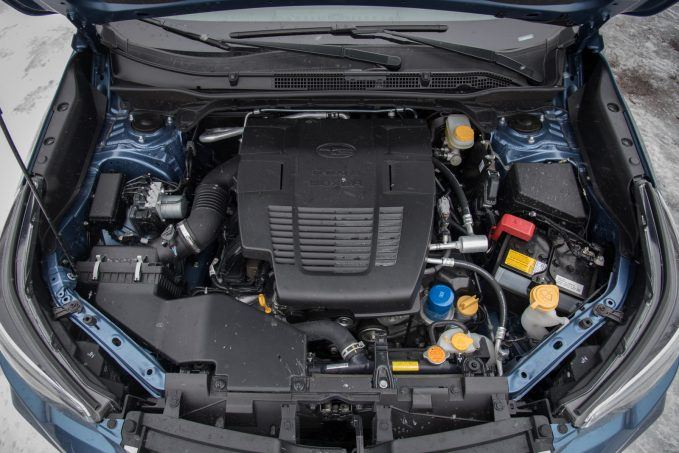
\includegraphics[width=0.25\linewidth]{engine}
        \end{tabular} & 
        \begin{tabular}{l}
            \parbox{0.65\linewidth}{
            R is like a car's engine. It is the program that powers your data analysis.
            }
        \end{tabular}
    \end{tabular} \\
    \vspace{1ex}
    \begin{tabular}{@{\extracolsep{-2ex}} c l}
        \begin{tabular}{c}
            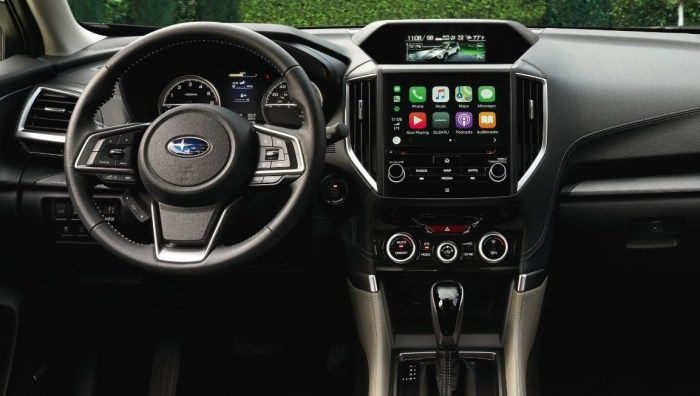
\includegraphics[width=0.25\linewidth]{dashboard}
        \end{tabular} & 
        \begin{tabular}{l}
            \parbox{0.65\linewidth}{
            RStudio is like a car's dashboard. It is the program you interact with to harness the power of your ``engine.''
            }
        \end{tabular}
    \end{tabular}
\end{frame}

\begin{frame}[fragile]\frametitle{Fundamentals of R}
    Everything is an object
\begin{knitrout}\footnotesize
\definecolor{shadecolor}{rgb}{0.969, 0.969, 0.969}\color{fgcolor}\begin{kframe}
\begin{alltt}
\hlstd{foo}
\end{alltt}
\end{kframe}
\end{knitrout}
    \vspace{3ex}
    Every object has a name and value
\begin{knitrout}\footnotesize
\definecolor{shadecolor}{rgb}{0.969, 0.969, 0.969}\color{fgcolor}\begin{kframe}
\begin{alltt}
\hlstd{foo} \hlkwb{<-} \hlnum{2}
\end{alltt}
\end{kframe}
\end{knitrout}
    \vspace{3ex}
    You use functions on objects
\begin{knitrout}\footnotesize
\definecolor{shadecolor}{rgb}{0.969, 0.969, 0.969}\color{fgcolor}\begin{kframe}
\begin{alltt}
\hlkwd{mean}\hlstd{(foo)}
\end{alltt}
\end{kframe}
\end{knitrout}
    \vspace{3ex}
    Functions come in packages/libraries
\begin{knitrout}\footnotesize
\definecolor{shadecolor}{rgb}{0.969, 0.969, 0.969}\color{fgcolor}\begin{kframe}
\begin{alltt}
\hlkwd{library}\hlstd{(mlogit)}
\end{alltt}
\end{kframe}
\end{knitrout}
\end{frame}

\begin{frame}[fragile]\frametitle{Playing Around in R}
    Basic math operations
\begin{knitrout}\footnotesize
\definecolor{shadecolor}{rgb}{0.969, 0.969, 0.969}\color{fgcolor}\begin{kframe}
\begin{alltt}
\hlnum{1} \hlopt{+} \hlnum{2}
\end{alltt}
\begin{verbatim}
## [1] 3
\end{verbatim}
\begin{alltt}
\hlnum{1} \hlopt{+} \hlnum{2} \hlopt{==} \hlnum{3}
\end{alltt}
\begin{verbatim}
## [1] TRUE
\end{verbatim}
\begin{alltt}
\hlstd{(}\hlnum{1} \hlopt{+} \hlnum{2}\hlstd{)} \hlopt{/} \hlnum{3}
\end{alltt}
\begin{verbatim}
## [1] 1
\end{verbatim}
\begin{alltt}
\hlnum{2}\hlopt{^}\hlnum{3}
\end{alltt}
\begin{verbatim}
## [1] 8
\end{verbatim}
\end{kframe}
\end{knitrout}
\end{frame}

\begin{frame}[fragile]\frametitle{Playing Around in R}
    Basic math with objects
\begin{knitrout}\footnotesize
\definecolor{shadecolor}{rgb}{0.969, 0.969, 0.969}\color{fgcolor}\begin{kframe}
\begin{alltt}
\hlstd{a} \hlkwb{<-} \hlnum{1}
\hlstd{b} \hlkwb{<-} \hlnum{2}
\hlstd{a} \hlopt{+} \hlstd{b}
\end{alltt}
\begin{verbatim}
## [1] 3
\end{verbatim}
\begin{alltt}
\hlstd{c} \hlkwb{<-} \hlstd{a} \hlopt{+} \hlstd{b}
\hlstd{c}
\end{alltt}
\begin{verbatim}
## [1] 3
\end{verbatim}
\begin{alltt}
\hlstd{(a} \hlopt{+} \hlstd{b)} \hlopt{/} \hlstd{c}
\end{alltt}
\begin{verbatim}
## [1] 1
\end{verbatim}
\begin{alltt}
\hlstd{b}\hlopt{^}\hlstd{c}
\end{alltt}
\begin{verbatim}
## [1] 8
\end{verbatim}
\end{kframe}
\end{knitrout}
\end{frame}

\begin{frame}[fragile]\frametitle{Playing Around in R}
    Functions
\begin{knitrout}\footnotesize
\definecolor{shadecolor}{rgb}{0.969, 0.969, 0.969}\color{fgcolor}\begin{kframe}
\begin{alltt}
\hlkwd{exp}\hlstd{(}\hlnum{2}\hlstd{)}
\end{alltt}
\begin{verbatim}
## [1] 7.389056
\end{verbatim}
\begin{alltt}
\hlkwd{sqrt}\hlstd{(}\hlnum{3}\hlstd{)}
\end{alltt}
\begin{verbatim}
## [1] 1.732051
\end{verbatim}
\begin{alltt}
\hlstd{d} \hlkwb{<-} \hlkwd{c}\hlstd{(}\hlnum{1}\hlstd{,} \hlnum{2}\hlstd{,} \hlnum{3}\hlstd{, a, b, c)}
\hlstd{d}
\end{alltt}
\begin{verbatim}
## [1] 1 2 3 1 2 3
\end{verbatim}
\begin{alltt}
\hlkwd{mean}\hlstd{(d)}
\end{alltt}
\begin{verbatim}
## [1] 2
\end{verbatim}
\begin{alltt}
\hlkwd{max}\hlstd{(d)}
\end{alltt}
\begin{verbatim}
## [1] 3
\end{verbatim}
\begin{alltt}
\hlkwd{min}\hlstd{(d)}
\end{alltt}
\begin{verbatim}
## [1] 1
\end{verbatim}
\end{kframe}
\end{knitrout}
\end{frame}

\begin{frame}[fragile]\frametitle{Playing Around in R}
    Matrix math
\begin{knitrout}\footnotesize
\definecolor{shadecolor}{rgb}{0.969, 0.969, 0.969}\color{fgcolor}\begin{kframe}
\begin{alltt}
\hlstd{mat_a} \hlkwb{<-} \hlkwd{matrix}\hlstd{(}\hlkwd{c}\hlstd{(}\hlnum{1}\hlstd{,} \hlnum{2}\hlstd{,} \hlnum{3}\hlstd{,} \hlnum{4}\hlstd{),} \hlkwc{nrow} \hlstd{=} \hlnum{2}\hlstd{)}
\hlstd{mat_a}
\end{alltt}
\begin{verbatim}
##      [,1] [,2]
## [1,]    1    3
## [2,]    2    4
\end{verbatim}
\begin{alltt}
\hlnum{2} \hlopt{*} \hlstd{mat_a}
\end{alltt}
\begin{verbatim}
##      [,1] [,2]
## [1,]    2    6
## [2,]    4    8
\end{verbatim}
\begin{alltt}
\hlstd{mat_a} \hlopt \hlstd{mat_a}
\end{alltt}
\begin{verbatim}
##      [,1] [,2]
## [1,]    7   15
## [2,]   10   22
\end{verbatim}
\end{kframe}
\end{knitrout}
\end{frame}

\begin{frame}[fragile]\frametitle{Playing Around in R}
    Install and load packages
\begin{knitrout}\footnotesize
\definecolor{shadecolor}{rgb}{0.969, 0.969, 0.969}\color{fgcolor}\begin{kframe}
\begin{alltt}
\hlkwd{install.packages}\hlstd{(}\hlkwd{c}\hlstd{(}\hlstr{'tidyverse'}\hlstd{,} \hlstr{'mlogit'}\hlstd{,} \hlstr{'gmm'}\hlstd{))}
\hlkwd{library}\hlstd{(tidyverse)}
\hlkwd{library}\hlstd{(mlogit)}
\hlkwd{library}\hlstd{(gmm)}
\end{alltt}
\end{kframe}
\end{knitrout}
\end{frame}

\begin{frame}\frametitle{Announcements}
    For next time
    \begin{itemize}
        \item Reiss and Wolack (2007), Sections 1--4
        \item Install R software
    \end{itemize}
\end{frame}

\end{document}
